\documentclass{article}
\usepackage{graphicx}
\begin{document}
\title{CS 124 Programming Assignment 3}
\author{30943147}
\maketitle

\section*{Dynamic Programming solution}
First, we sum up all of the numbers in our input array nums. Let $S = \lceil \frac{sum}{2} \rceil$. Now, we create a two dimensional array of booleans $P$. $P$ has dimensions $n+1 \times S$, where $n$ is the length of our input array. $P[i][j]$ will be true if some subset of the first $i$ entries of nums (our input array) sums to $j$. We initialize $P[0][j \neq 0]$ to false since no elements cannot sum to anything other than 0. We initialize $P[i][0]$ to true since for any set of $i$ elements, the empty subset will sum to 0. Now we diagonally fill in $P$ as follows:

There are two conditions under which P[i][j] will be true. If neither is met, set P[i][j] to false. The first case is that the $i^{th}$ element is not in the subset and therefore does not contribute to the sum, in which case $P[i][j]$ should be true if $P[i-1][j]$ is true. The second case is that the $i^{th}$ element is in the subset. Then $P[i][j]$ should be true if the previous $i-2$ elements of nums sum to to $j-nums[i-1]$. (The indices for $i$ in P are 1 ahead of the indices for $i$ in nums since P[0] corresponds to no elements of nums being included). This corresponds to setting $P[i][j]$ to true if $P[i-1][j-nums[i-1]]$ is true. When coding we would check that $j-nums[i-1] \geq 0$ before trying to index into $P$, and ignoring this step otherwise. 

Once we have filled out our array, we want to return the residue that corresponds to the subset of elements whose sum $j$ is closest to $S$. That residue will be equal to $S-2*j$. To do so, we iterate through all $P[n][j]$ starting from $j=S$ and returning $S-2*j$ as soon as we find $P[n][j] = $ true.

\subsection*{DP Runtime}
The runtime of that dynamic programming solution is $O(S * n)$, where $S$ half the sum of the elements rounded up, and $n$ is the number of elements. This is pseudopolynomial since $S$ polynomial in the value of the input (ie the set of numbers of the array) but exponential in the length of the input, since a $b$ bit number can have value on the order of $2^b$. This is the definition of pseudopolynomial runtime. 

\section*{Results}
All results here were run over the same set of 100 input files each containing 100 randomly generated integers in the range $[1, 10^{12}]$. The files were generated by geninfile.java. 
\subsection*{Karmarker-Karp}
Average residue: 243484\\
Standard deviation: 329181
\subsection*{Heuristics without Prepartitioning}
\begin{center}
\begin{tabular}{| c | c | c |}
\hline
Heuristic & Avg & Stdev \\
\hline\hline
RR & 328969027 & 349722426 \\
\hline
HC & 14255150660 & 15999889638\\
\hline
SA & 10940824994 & 11648602710 \\
\hline
Repeated random performs significantly better than simulated annealing, which performs slightly better than hill climbing. 
\end{tabular}
\end{center}
\subsection*{Heuristics with Prepartitioning}

\begin{center}
\begin{tabular}{| c | c | c |}
\hline
Heuristic & Avg & Stdev \\
\hline\hline
RR & 164 &  144\\
\hline
HC & 833 & 808\\
\hline
SA & 181 &  180\\
\hline

\end{tabular}
\end{center}
This chart displays the results for the 3 heuristics, wtih the trials sorted in order of increasing residue for each heuristic and placed in a graph. \\
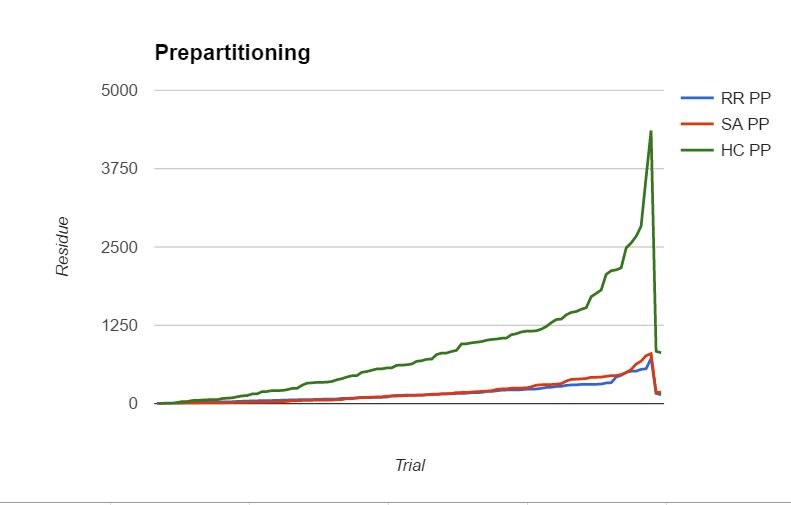
\includegraphics[scale=0.5]{prepartitioning.jpg}

Prepartitioning reduced the residue by many orders of magnitude, and the difference made by using prepartitioning far outweight the difference between specific heuristics. The ordering of $RR < SA < HC$ was the same with and without prepartitioning, but using prepartitioning brought the residues for SA much closer to RR than to HC. I was surprised by how high the standard deviation was for all of the heuristics, with and without partition. Despite the high standard deviation between files, the average seemed pretty stable when I ran the randomized algorithms over all files multiple times. Running the same heuristic over the same file multiple times could produce significantly different answers, however. The differences were most noticeable for the hill climbing algorithm. I suspect this was because hill climbing has the flaw that it can get stuck in local minima, and on the trials that produced high residue it did so. 

I was impressed by how low the residues were using the prepartitioning given how large the input numbers are--a few trials had residues as low as 1!


\section*{KK as a starting point}
It seems promising to try using the solution returned by the initial run of Karmarker-Karp as a starting point for the various random heuristics, rather than starting with a randomly generated solution $S$ and trying to optimize it, since the solution provided by Karmarker-Karp will be on average much better than a random starting point (in my results it is several orders of magnitude better). This would be especially promising for the two local search heuristics, hill climbing and simulated annealing.  

\section*{Runtime}
Runtime is done over 100 different sets of input numbers with max iter set to 25000.
\begin{center}
\begin{tabular}{ | c | c |}
\hline
 & Runtime \\
\hline\hline
KK & 14.5s \\
\hline
RR standard & 25s \\
\hline
HC standard & 16s\\
\hline
SA standard & 17s\\
\hline
RR prepartitioning & 1m11s\\
\hline
HC prepartitioning & 58.4s\\
\hline
SA prepartitioning & 1m3s\\
\hline
\end{tabular}
\end{center}
Runtimes are higher with prepartitioning than without because Karmarker-Karp takes $O(n \log n)$. Runtime seems pretty comparable between hill climbing and simulated annealing, with repeated random taking slightly longer in both standard representation and prepartioning. This makes sense, since for both solution representations it takes more work to generate an entirely new random solution than to merely generate a neighbor. 

\section*{Code Design}
\subsection*{Randomness}
Java's default random number generators do not generate all long integers. ThreadLocalRandom, a random number generator built into each thread, does, and so I used that. This is why threads occasionally come up in my code even though there is only one thread--it was the best random number generator I could find. 
\subsection*{Modes}
I made the main method take an additional argument to specify which heuristic we are testing, and have the kk script automatically supply it so that ./kk nums.txt would work as in the spec. This resulted in a lot of different scripts to test the different heuristics, which made it easier for me to test and time them separately.  
\end{document}